\scanpage{137}
\[
R^{\unsure{*|\alpha}}(if)_*\Longleftarrow R^pi_*(R^qf_*(Q_l))
\]
\figure{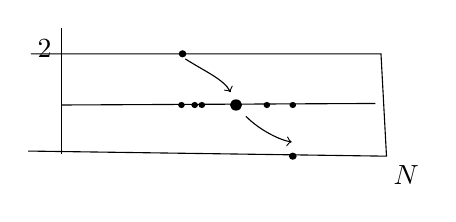
\begin{tikzpicture}[x=.7cm,y=.65cm]
\draw (0,.05)--(0,2.5);
\draw (-.55,2)--(5.8,2)--(5.9,0)--(-.6,.1);
\draw (0,1)--(5.7,1.03);
\node[left] at (0,2.1) {2};
\node[below right] at (5.85,0) {\(N\)};
\fill (2.2,2) circle (.07);
\foreach \x in {2.18,2.42,2.55,3.17,3.73,4.2}
{\fill (\x,1) circle (.06);}
\fill (3.17,1) circle (.11);
\fill (4.2,0) circle (.07);
\draw[->] (2.25,1.9)..controls (2.6,1.66) and (2.95,1.5)..(3.07,1.25);
\draw[->] (3.35,.78)..controls (3.6,.5) and (4,.3)..(4.18,.28);
\end{tikzpicture}}

avec \(E_2^{pq}=0\) si \(q\notin[0,2]\).
D'ailleurs \(R^0f_*(Q_l)\) est essentiellement \(Q_l\)
(du moins si \(f\) à fibres connexes, \unsure{ce que}
\unsure{l'on se ramène facilement}...],
donc les \deleted{\(R^pi_*\) sont} \(E_2^{p0}\) sont
\((d-1)\)-admissibles par \deleted{l'hyp.} ce qui vient d'être prouvé.

\deleted{Donc} D'autre part \(R^2f_*(Q_l)\simeq Q_l(-1)\), et
\[
E_2^{p2}\simeq R^pi_*(R^2f_*(Q_l))
\simeq\deleted{\unsure{E_2^{p2}}}
\inserted{Q_l(-1)}\deleted{\unsure{R^pi_*}}\otimes E_2^{p0}
\]
est donc également \((d-1)\) admissible, à fortiori
\deleted{\(\unsure{(d+d')}\)}
\inserted{\((d+d'-1)\)-}admissible
\inserted{i.e. \(d\)-admissible},
\deleted{Pour} On en conclut, utilisant lemme 2,
\inserted{et la constructibilité des \(E_2^{pq}\),}
que \(E_2^{p1}\) est une extension de \deleted{deux}\inserted{trois} faisceaux,
les extrêmes étant \deleted{\((d+d'-1)\)-\unsure{ad}} \(d\)-admissibles,
et le médian \unsure{des|est}
\[
E_3^{p1}=\cdots=E_\infty^{\unsure{p1|pq}}.
\]
Il suffit donc de prouver que \(E_\infty^{\unsure{p1|pq}}\) est \(d\)-admissible,
ou encore que \(R^n(if)_*(Q_l)\) l'est, ou encore que
\(R^n(gj)_*(\unsure{Q_l|Y})\) l'est,
ce qui par Leray et lemme 3 nous ramène au cas des
\(R^nj_*(Q_l)\), qui sont traités...
% archive foliation: 136
